\documentclass[problem]{mcs}

\begin{pcomments}
  \pcomment{PS_koch_induction}
  \pcomment{elaboration of PS_koch_snowflake}
  \pcomment{ARM \& CH, 4/11/14}
\end{pcomments}

\pkeywords{
  induction
  equilateral
  recurrence
  geometric
  sum
}

%%%%%%%%%%%%%%%%%%%%%%%%%%%%%%%%%%%%%%%%%%%%%%%%%%%%%%%%%%%%%%%%%%%%%
% Problem starts here
%%%%%%%%%%%%%%%%%%%%%%%%%%%%%%%%%%%%%%%%%%%%%%%%%%%%%%%%%%%%%%%%%%%%%

\begin{problem}
Here is an interesting construction of a geometric object known as the
\emph{Koch snowflake}.  Define a sequence of polygons $S_0, S_1$
recursively, starting with $S_0$ equal to an equilateral triangle with
unit sides.  We construct $S_{n+1}$ by removing the middle third of
each edge of $S_n$ and replacing it with two line segments of the same
length, as illustrated in Figure~\ref{kochind}.

\begin{figure}[h]
  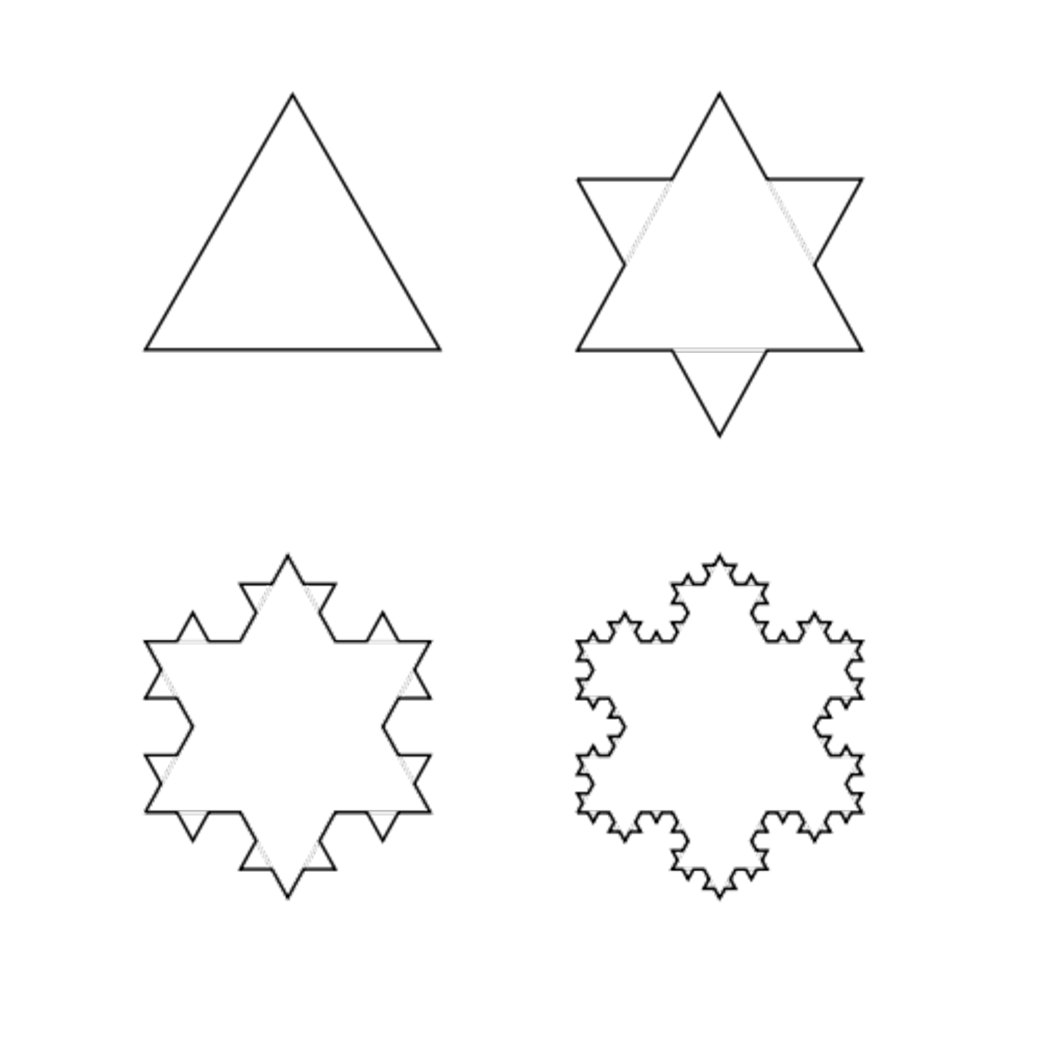
\includegraphics[width=2.5in]{koch_full}
  \caption{$S_0,S_1,S_2 \text{ and } S_3$.}
  \label{kochind}
\end{figure}

Let $a_n$ be the area of $S_n$.  Observe that $a_0$ is just the area
of the unit equilateral triangle which by elementary geometry is
$\sqrt{3}/4$.

Prove by induction that for $n \geq 0$, the area of the $n^{\text{th}}$
 snowflake is given by:
\begin{equation}\label{an1s3}
  a_n = a_0 \paren{\frac{8}{5} - \frac{3}{5} \paren{\frac{4}{9}}^n}.
\end{equation}

\begin{staffnotes}
\hint  If need be, prompt for the recurrence~\eqref{an+1a}.
\end{staffnotes}


\begin{solution}
Let $l_n$ be the length of the edges in $S_n$, and $e_n$ be the number
of edges in $S_n$.  So $l_0=1$ and $e_0=3$.  From the definition of
$S_{n+1}$, we have
\begin{align}
l_{n+1} & = l_n/3,\notag\\ %\label{ln+13}
e_{n+1} & = 4e_n,\notag\\  %\label{en+14}
a_{n+1} & = a_n + e_n \cdot a_0 \paren{l_{n+1}}^2.\label{an+1a}
\end{align}
The last equation arises since the area of an equilateral triangle
with edge length $l$ is $a_0 l^2$.

Clearly,
\begin{equation}\label{ln13nen}
l_n = (1/3)^{n} \qquad \text{and}\qquad e_n = 3 \cdot 4^{n},
\end{equation}
as can be verified by a trivial induction.

We now use~\eqref{an+1a} to prove by induction on $n$
that~\eqref{an1s3} holds for all $n \geq 0$, with~\eqref{an1s3}
serving as Induction Hypothesis.

\begin{proof}
\inductioncase{Base case}: ($n=0$).  The right-hand side
of~\eqref{an1s3} simplifies to $a_0$ when $n=0$.

\inductioncase{Induction step}: Assume the Induction Hypothesis is
true for some nonnegative integer $n$.
\iffalse
That is,
\begin{equation}\label{85indhyp}
 a_m =  a_0 \paren{\frac{8}{5} - \frac{3}{5} \paren{\frac{4}{9}}^m} .
\end{equation}
\fi

From~\eqref{an+1a}, we have:
\begin{align}
a_{n+1} & = a_n + 3 \cdot 4^{n} \cdot a_0 \cdot \paren{(1/3)^{n+1}}^2 & \text{(by~\eqref{ln13nen})}\notag\\
%      & = a_n + a_0  \cdot 3 \cdot 4^{n} (1/9)^{n+1}\notag\\
      & = a_n + a_0 \cdot \frac{1}{3} \cdot \paren{\frac{4}{9}}^{n} \label{am+a031949}\\
      & = a_0 \paren{\frac{8}{5} - \frac{3}{5} \paren{\frac{4}{9}}^{n}}
      + a_0 \cdot \frac{1}{3} \cdot \paren{\frac{4}{9}}^{n} & \text{(by induction hypothesis~\eqref{an1s3})}\notag\\
      & = a_0 \paren{\frac{8}{5} +
                \paren{\frac{1}{3}  - \frac{3}{5}}  \paren{\frac{9}{4}}\paren{\frac{4}{9}}^{n+1}}\notag\\
%      & = a_0 \paren{\frac{8}{5} -
%                \paren{\frac{4}{3 \cdot 5}} \paren{\frac{9}{4}} \paren{\frac{4}{9}}^{n+1}}\notag\\
      & = a_0 \paren{\frac{8}{5} - \frac{3}{5} \paren{\frac{4}{9}}^{n+1}}\notag
\end{align}
which proves the Induction Hypothesis for $n+1$. 

\end{proof}
So as $n$ goes to infinity, the area $a_n$ approaches $8/ 5$ while the
perimeter approaches a nowhere differentiable curve whose length is
$\lim_{n \to \infty} e_n l_n = \lim_{n \to \infty} 3 \cdot (4/3)^n =
\infty$.

By the way, we derived~\eqref{an1s3} in the first place using the
formula for a geometric sum:
 \begin{align*}
 a_n & = a_{n-1} +  (a_0/3) \paren{\frac{4}{9}}^{n-1} & \text{(from \eqref{am+a031949})}\\
     & = a_{n-2} + (a_0/3) \paren{\frac{4}{9}}^{n-2}
                + (a_0/3) \paren{\frac{4}{9}}^{n-1} = \dots\\
     & = a_0 + (a_0/3) \sum_{k=0}^{n-1} \paren{\frac{4}{9}}^k\\
     & = a_0 \paren{1 + \frac{(1/3)(1- (4/9)^n)}{1-4/9}},
%     & = a_0 \paren{1 + \frac{(1/3)(1- (4/9)^n)}{5/9}}\\
%     & = a_0 \paren{\frac{8}{5} - \frac{3}{5}\paren{\frac{4}{9}}^n}
 \end{align*}
which simplifies to~\eqref{an1s3}.

\end{solution}

\end{problem}

%%%%%%%%%%%%%%%%%%%%%%%%%%%%%%%%%%%%%%%%%%%%%%%%%%%%%%%%%%%%%%%%%%%%%
% Problem ends here
%%%%%%%%%%%%%%%%%%%%%%%%%%%%%%%%%%%%%%%%%%%%%%%%%%%%%%%%%%%%%%%%%%%%%

\endinput

